\documentclass{article}
\usepackage{amsthm}
\usepackage{comment}
\usepackage{amsmath}
\usepackage{amsfonts}
\usepackage{sectsty}
\usepackage{hyperref}
\usepackage{fancyhdr}
\usepackage[top=1in,bottom=1in,left=1in,right=1in]{geometry}
\usepackage{float}
\usepackage{graphicx}
\usepackage{tabularx}
\usepackage{mathtools}

\newtheorem{theorem}{Theorem}
\newtheorem{corollary}{Corollary}[theorem]

\title{Lecture 3 - Analysis of Sets}
\author{Matthew Farah, \href{mailto:farahm11@mcmaster.ca}{$\langle$farahm11@mcmaster.ca$\rangle$}, 400468251}
\date{\today}

%FIX: FLESH OUT PROOFS

\hypersetup{
        colorlinks=true,
        linkcolor=blue,
        filecolor=magenta,
        urlcolor=blue,
        citecolor=blue,
	anchorcolor=blue
}

\fancyhead{}
\fancyhead[L]{Matthew Farah, \href{mailto:farahm11@mcmaster.ca}{$\langle$farahm11@mcmaster.ca$\rangle$}, 400468251}
\fancyhead[R]{Lecture 3 - Analysis of Sets}

\newenvironment{directsubsubs}{
  \makeatletter
  \renewcommand\thesubsubsection{\thesection.\Roman{subsubsection}}
  \makeatother
}{
  \makeatletter
  \renewcommand\thesubsubsection{\thesubsection.\Roman{subsubsection}}
  \makeatother
}

\renewcommand{\thesubsection}{\thesection.\alph{subsection}}
\renewcommand{\thesubsubsection}{\thesection.\alph{subsection}.\Roman{subsubsection}}
\makeatletter

\sectionfont{\fontsize{12}{12}\bfseries}
\subsectionfont{\fontsize{10}{12}\normalfont}
\subsubsectionfont{\fontsize{10}{12}\normalfont}

\begin{document}

\maketitle
\pagestyle{fancy}

\begin{theorem}
	The set $\mathbb{N} \times \mathbb{N} = \{(n, m) \; | \; n, m \in \mathbb{N}\}$ is denumerable.
\end{theorem}

\begin{proof}

	Informally, we can show this with a diagonalization proof:

	\begin{figure}[H]
		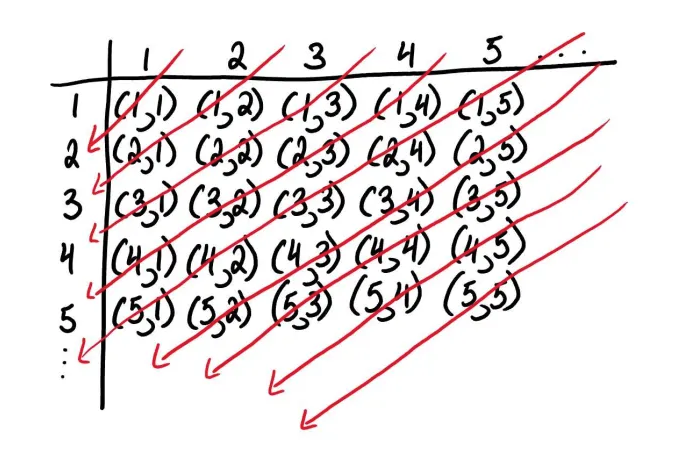
\includegraphics[width=\linewidth]{./imgs/NxN-Diagonalization-Argument.png}
		\caption{Diagonalization argument for countability of $\mathbb{N} \times \mathbb{N}$}
	\end{figure}

	Here, each entry in the table corresponds to an element of the set $\mathbb{N} \times \mathbb{N}$. Since we are able to draw a line (the red arrows), which crosses through each element in the set exactly once, this informal proof shows us that there exists a bijective function between $\mathbb{N}$ and $\mathbb{N} \times \mathbb{N}$.

\end{proof}

\begin{corollary}
	The set $\mathbb{Q}$ is denumerable.
\end{corollary}

\begin{proof}
	The proof for the denumerability of $\mathbb{Q}$ can be demonstrated with a diagonalization argument much in the same way as the proof for $\mathbb{N} \times \mathbb{N}$.


\end{proof}

\begin{theorem}
	Russel's Paradox: There does not exist a set of all sets.
\end{theorem}

\begin{proof}
Assume, for the purposes of contradiction, that there exists a set of all sets. Then, in such a set, there must exist a set $A$ which contains all sets which do not contain themselves. Now, if $A$ does not contain itself, then $A$ is a set which does not contain itself and thus must belong to $A$. But then, if $A$ is not contained in $A$, then $A$ is a set which does not contain itself and therefore should be in $A$. This is necessarily a contradiction and thus no such set can exist
\end{proof}

\begin{itemize}
	\item The implication of Russell's paradox is that there must exist certain requirements on what can and cannot be a set.
\end{itemize}

\begin{itemize}
	\item For two sets $A$ and $B$, $B$ is a \emph{subset} of $A$ if $b \in B \implies b \in A$.
	\begin{itemize}
		\item Alternatively, we can call $A$ a \emph{superset} of $B$.
	\end{itemize}
	\item For a set $A$, the power set of $A$ is the set of all subsets of $A$.
	\begin{itemize}
		\item Denoted $\wp(A)$.
	\end{itemize}
\end{itemize}

\begin{theorem}
	Cantor's Theorem: For any set $A$, there exists not surjective function $f$ such that $f: A \rightarrow \wp(A)$.
\end{theorem}

\begin{proof}
	We begin by separating our proof into 2 cases depending on the cardinality of $A$.
	
	\begin{center}
		\large{\underline{If $A$ is finite}}
	\end{center}
	Between two finite sets $A$ and $B$, there can exist no surjection from $A$ to $B$ if $\#A < \#B$.
	If $A$ is finite, then we know there exists a bijection between $A$ and $\mathbb{N}_n$ for some $n \in \mathbb{N}$, making the cardinality of $A$ n. The cardinality of the power set of $A$ is therefore given by $2^n$ (since $\forall a \in A$, we have a binary choice between whether to include it or not in a given subset of $A$).

	Using this, we know that there can exist no surjection from $A$ to $\wp(A)$ if $\#A < \#\wp(A)$. Since $\#A = n$ and $\#\wp(A) = 2^n$, we need to prove $P(n): n < 2^n$ is true $\forall n \in \mathbb{N}$, which we do by induction.

	\begin{center}
		\underline{(1) Prove the base case (Show $P(1)$ is true).}
	\end{center}

	\begin{align*}
		&\text{LHS:}& &\text{RHS:} \\
		&n & &2^n \\
		&=1& &=2^1 \\
		&=1& &=2 \\
	\end{align*}

	Therefore, since $LHS < RHS$, $P(1)$ is true.

	\begin{center}
		\underline{(2) Formulate the induction hypothesis (State $P(k)$).}
	\end{center}
	
	\begin{align*}
		P(k): k < 2^k \\
	\end{align*}

	\begin{center}
		\underline{(3) Prove $P(k) \implies P(k + 1)$}
	\end{center}
	\begin{align*}
		&k + 1 \\
		&<2^{k} + 1 \\
		&<2^{k + 1} \\
	\end{align*}
	Therefore, since $P(1)$ is true and $P(k) \implies P(k + 1)$, by the principle of mathematical induction, $P(n)$ is true $\forall n \in \mathbb{N}$.

	Thus, our proof for finite $A$ is complete, since $\# A = 2 < 2^n = \#\wp(A)$ implies there can exist not surjective function from $A$ to $\wp(A)$.
	\begin{center}
		\underline{If $A$ is infinite}
	\end{center}
\end{proof}

\begin{corollary}
	If $A$ is denumerable then $\wp(A)$ is uncountable.
\end{corollary}

\end{document}
